\section{Appendix: pseudocode and flowcharts} \label{section: appendix}
This appendix provides the full blocks of pseudocode and its flowcharts.

{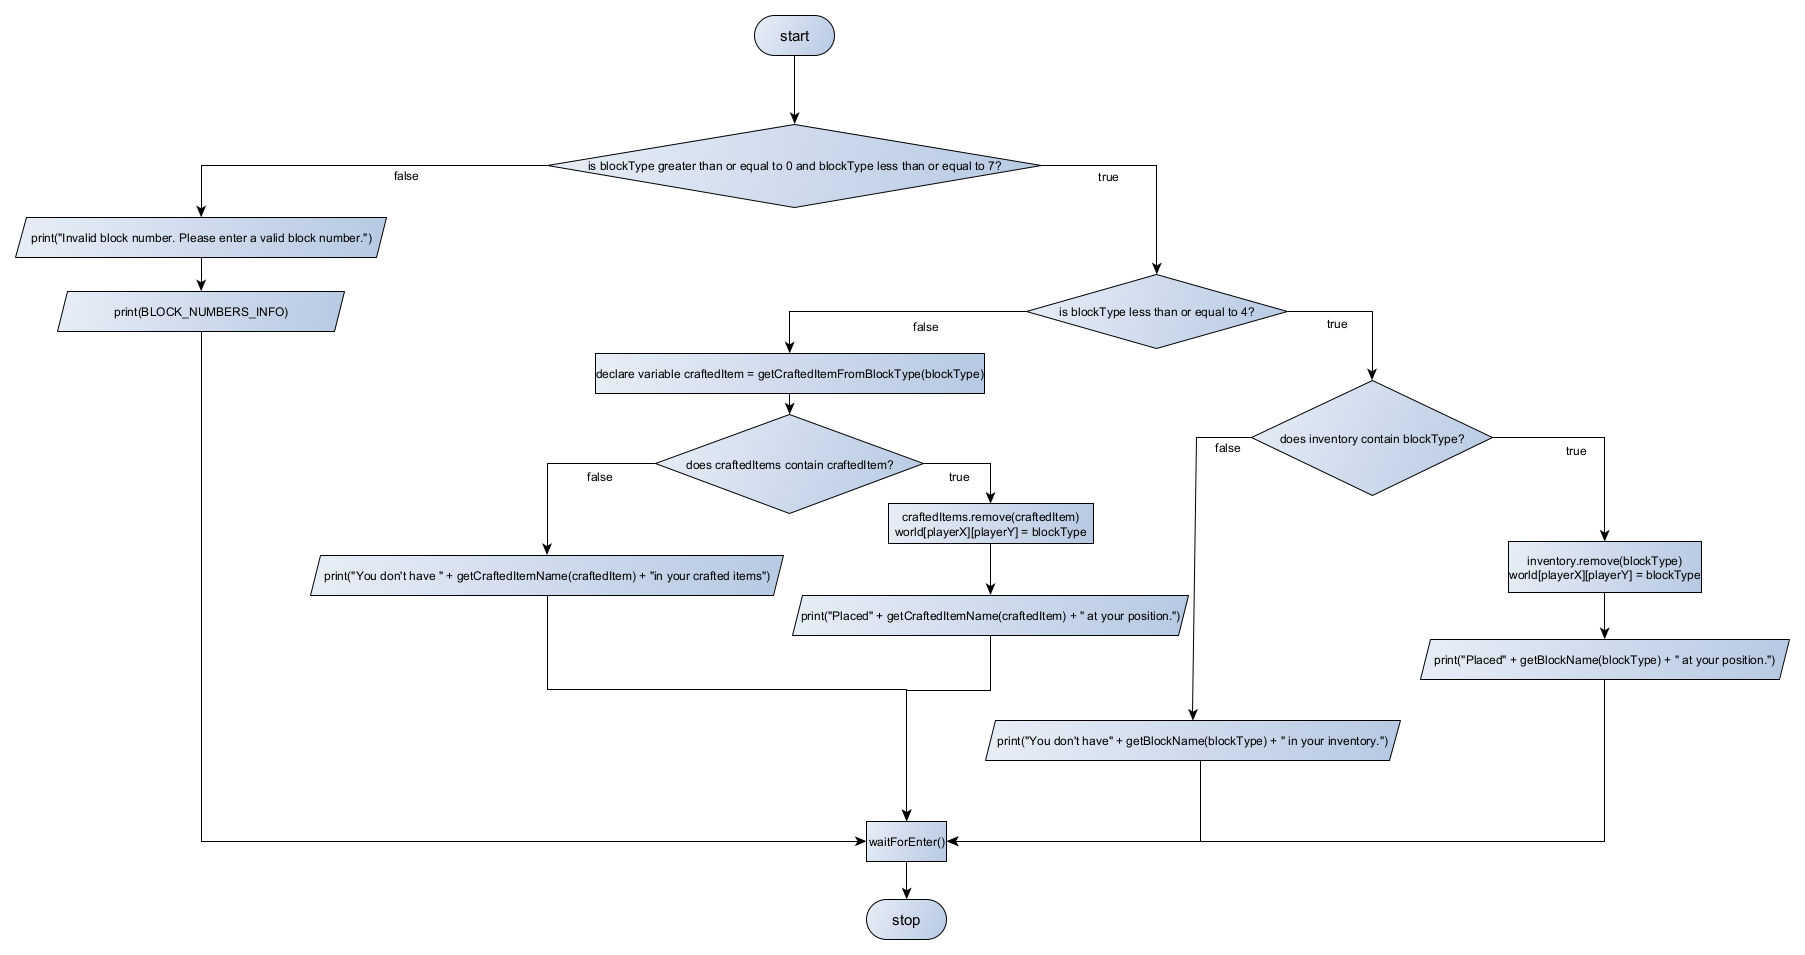
\includegraphics[width=\textwidth]{../flowchart/placeBlock.png}}

\begin{lstlisting}
function placeBlock(blockType)

if blockType is greater than or equal to 0 and blockType is less than or equal to 7 then 
	if blockType less than or equal to 4 then
		if inventory contains blockType then
			inventory.remove(blockType)
			world[playerX][playerY] = blockType
			print("Placed" + getBlockName(blockType) + " at your position.")

		else print("You don't have " + getBlockName(blockType) + " in your inventory")
		end if
	else
		craftedItem = getCraftedItemFromBlockType(blockType)
		if craftedItems contains craftedItem then 
			craftedItems.remove(craftedItem)
			world[playerX][playerY] = blockType
			print("Placed" + getCraftedItemName(craftedItem)+ " at your position.")
		else print("You don't have " + getCraftedItemName() + " in your inventory.")
		end if
	end if
else print("Invalid block number. Please enter a valid block number.")
print(BLOCK_NUMBERS_INFO)
end if
waitForEnter()
end function
\end{lstlisting}
\newpage

{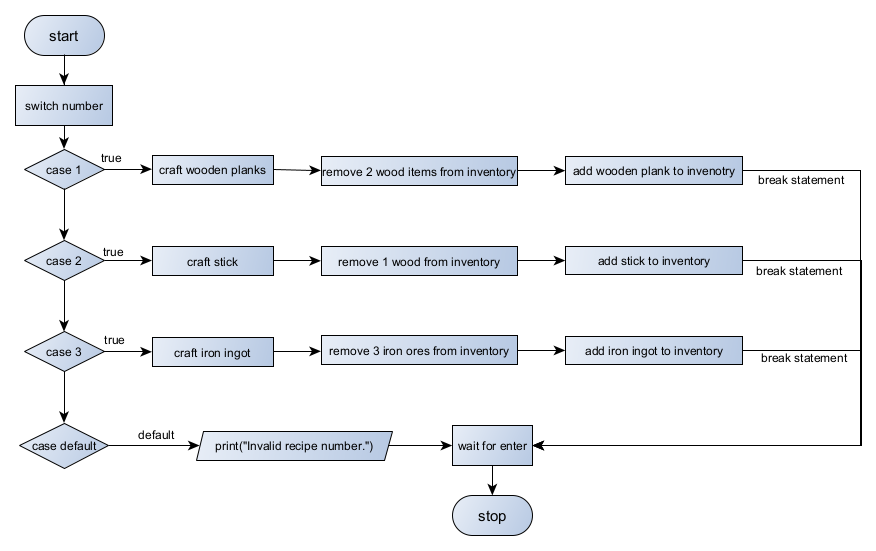
\includegraphics[width=\textwidth]{../flowchart/craftItem.png}}
\begin{lstlisting}
function craftItem(recipe)

switch(recipe)
case 1: 
	craftWoodenPlanks()
end if
case2: 
	craftStick()
end if
case3:
	craftIronIngot()
end if
default: 
	print("Invalid recipe number.")
end switch
waitForEnter()
end function
\end{lstlisting}
\newpage

{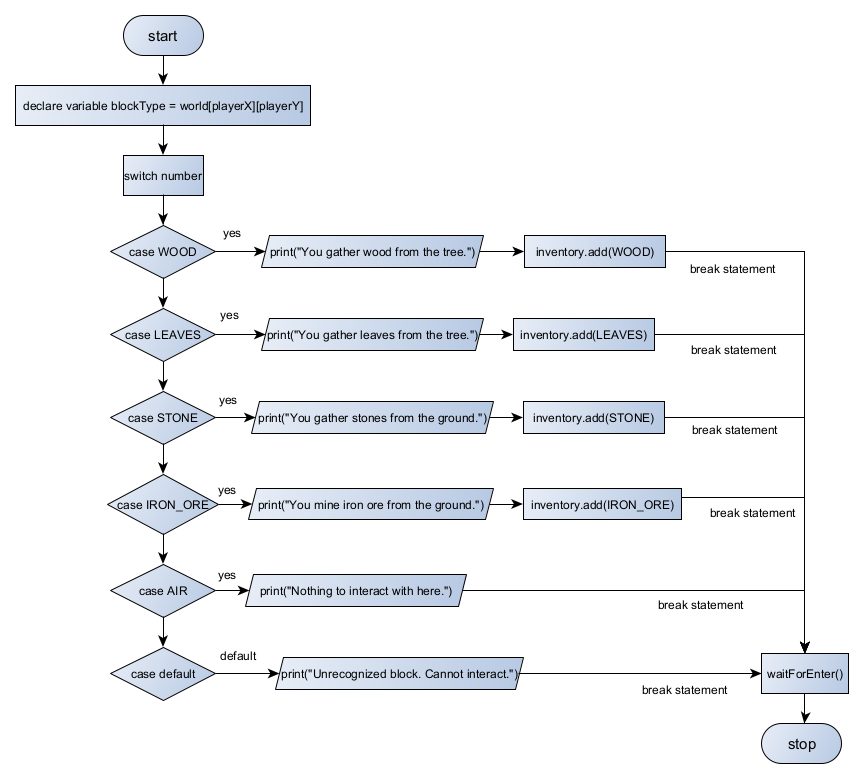
\includegraphics[width=\textwidth]{../flowchart/interactWithWorld.png}}


\begin{lstlisting}
function interactWithWorld()

blockType = world[playerX][playerY]
switch(blockType):
case WOOD: 
	print("You gather wood from the tree.")
	inventory.add(WOOD)
end if
case LEAVES:
	print("You gather leaves from the tree.")
	inventory.add(LEAVES)
end if
case STONE:
	print("You gather stones from the ground.")
	inventory.add(STONE)
end if
case IRON_ORE:
	print("You mine iron ore from the ground.")
	inventory.add(IRON_ORE)
end if
case AIR:
	print("Nothing to interact with here.")
end if
default: print("Unrecognized block. Cannot interact.")
end switch
waitForEnter()
end function
\end{lstlisting}
\newpage

{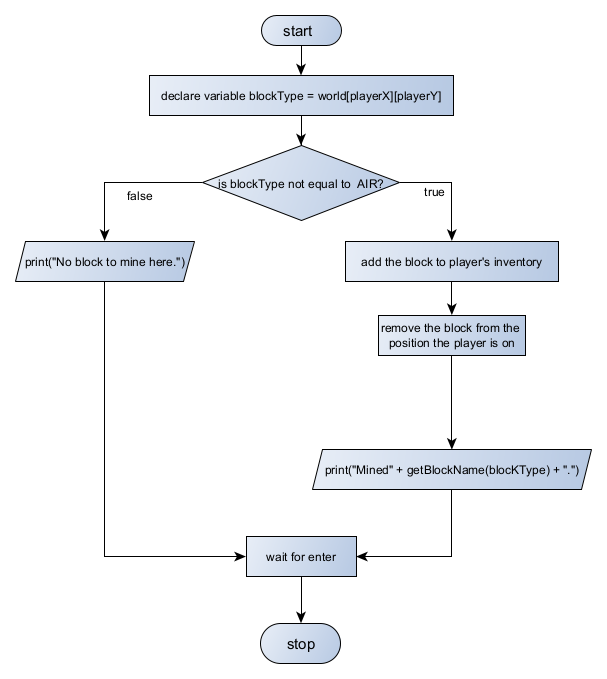
\includegraphics[width=\textwidth]{../flowchart/mineBlock.png}}
\begin{lstlisting}
function mineBlock()

blockType = world[playerX][playerY]
if blockType is not equal to AIR then 
	inventory.add(blockType)
	world[playerX][playerY] = AIR
	print("Mined " + getBlockName(blockType) + ".")
else print("No block to mine here.")
end if
waitForEnter()
end function
\end{lstlisting}
\newpage
{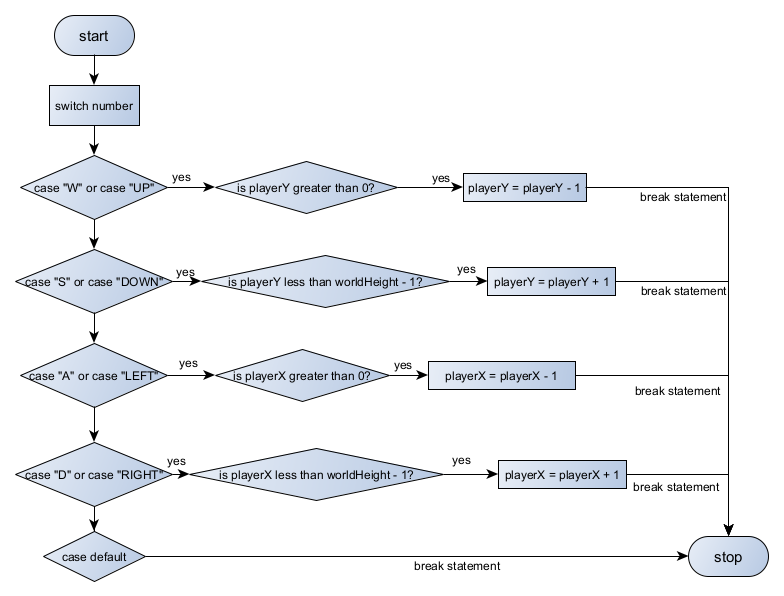
\includegraphics[width=\textwidth]{../flowchart/movePlayer.png}}
\begin{lstlisting}
function movePlayer(direction):

direction = uppercase(direction) //converts direction to uppercase for consistency
switch(direction):
case "W" or "UP":
	if playerY > 0 then playerY = playerY - 1
	end if
case "S" or "DOWN":
	if playerY < worldHeight - 1 then playerY = playerY + 1
	end if
case "A" or "LEFT":
	if playerX > 0 then playerX = playerX - 1
	end if
case "D" or "RIGHT":
	if playerX < worldWidth - 1 then playerX = playerX + 1
	end if
default: //do nothing
end switch
end function
\end{lstlisting}
\newpage

{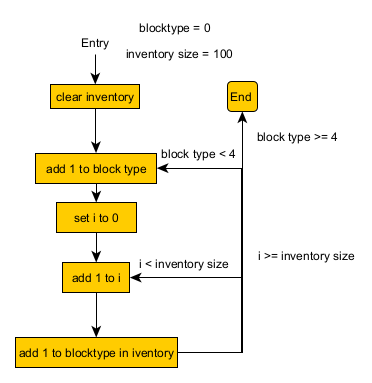
\includegraphics[width=\textwidth]{../flowchart/fillInventory.png}}
\begin{lstlisting}
function fillInventory()

blocktype = 0
inventory size = 100
clear inventory
if block type < 4
add 1 to block type
set i to 0
if i < inventory size
   add 1 to i
   add 1 blocktype in inventory

\end{lstlisting}
\newpage
{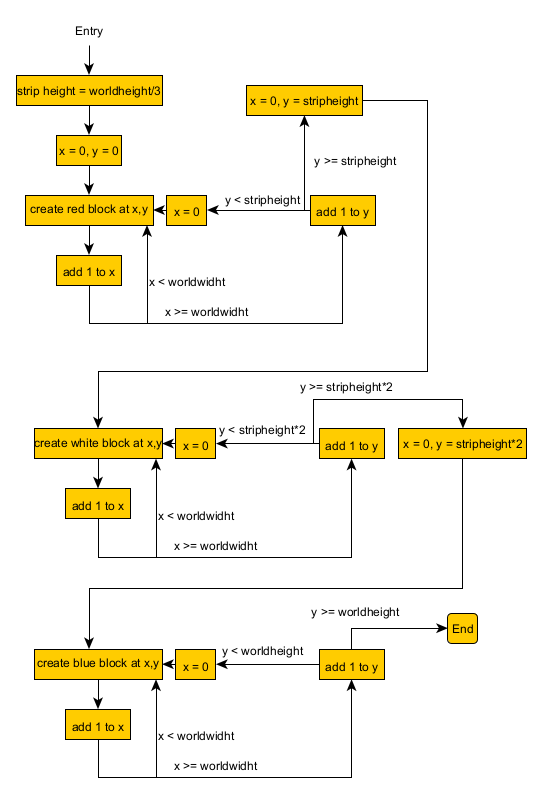
\includegraphics[width=\textwidth]{../flowchart/generateEmptyWorld.png}}
\begin{lstlisting}
function generateEmptyWorld()

redBlock = 1
whiteBlock = 4
blueBlock = 3

stripheight = world height / 3

y = 0
if y < stripheight(
   if x < worldwidth(
        
	create redblock at x, y
	add 1 to x
     )
    add 1 to y)

y = stripheight
if y < stripheight*2(
   if x < worldwidth(
        
	create redblock at x, y
	add 1 to x
     )
    add 1 to y)

y = stripheight*2
if y < worldheight(
   if x < worldwidth(
        
	create redblock at x, y
	add 1 to x
     )
    add 1 to y)
\end{lstlisting}
\newpage
{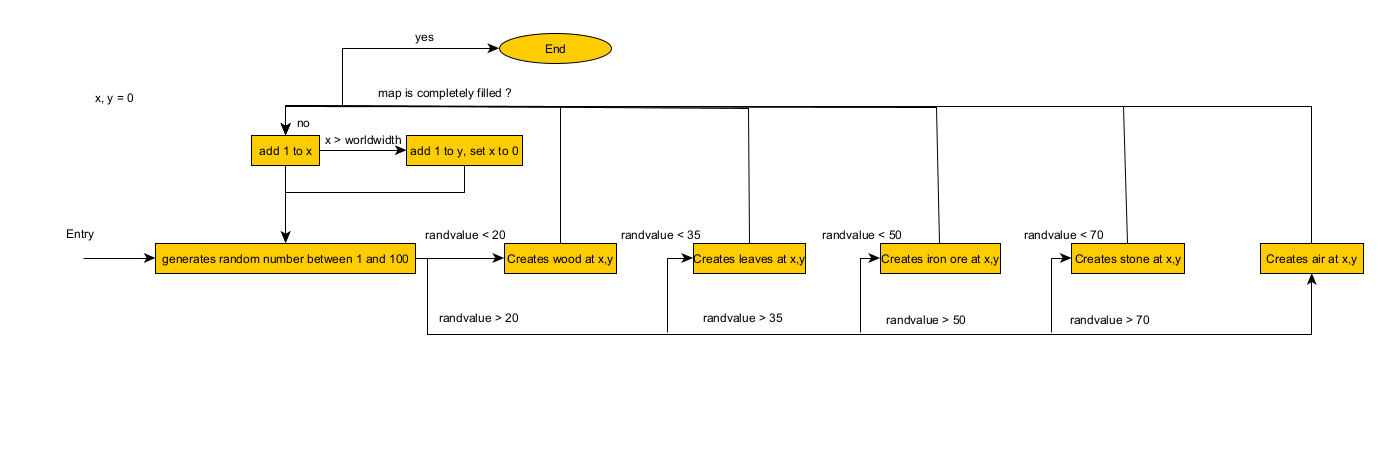
\includegraphics[width=\textwidth]{../flowchart/generateWorld.png}}
\begin{lstlisting}
function generateWorld()

x = 0
y = 0
if y < worldheight  
    if x < worldwidth 
        creates random number between 1 and 100
        if random number < 20
            creates wood at x, y
        else if random number < 35
            creates leaves at x, y
        else if random number < 50
            creates stone at x, y
        else if random number < 20
            creates iron ore at x, y
        else create air at x, y
    add 1 to x
add 1 to y

\end{lstlisting}
\newpage
{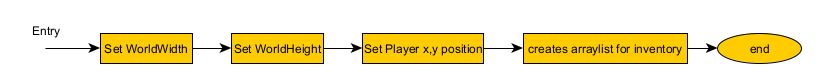
\includegraphics[width=\textwidth]{../flowchart/initGame.png}}
\begin{lstlisting}
function initgame()

set worldwidth
set worldheight
set world = [worldwidht][worldheight]
set playerx = worldwidght / 2
set playery = worldheight / 2
creates arraylist inventory

\end{lstlisting}
\newpage
{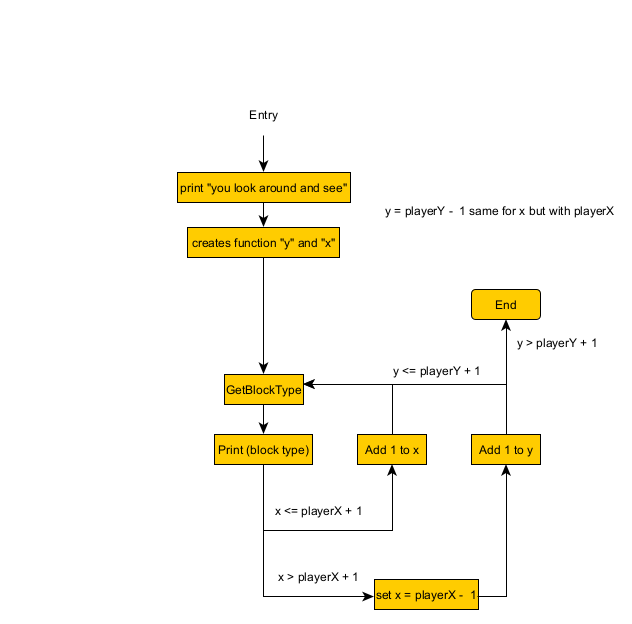
\includegraphics[width=\textwidth]{../flowchart/lookAround.png}}
\begin{lstlisting}
function lookAround()

print "You look around and see:"

set x = player x -1 , y = player y - 1
if y <= player Y + 1 
if x <= player X + 1
  get block type (x, y)
  print (block type)
else set x to player x - 1
     add 1 to y

\end{lstlisting}
\newpage

{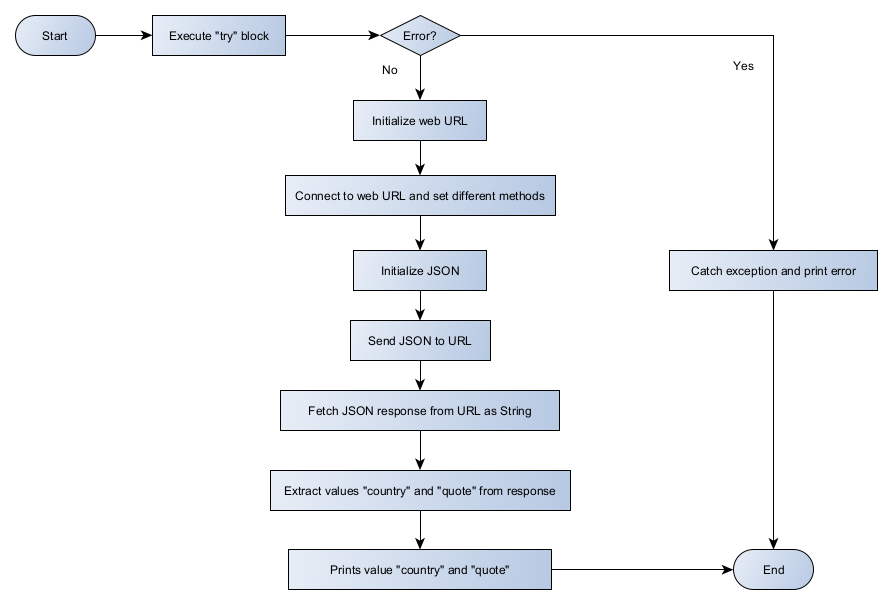
\includegraphics[width=\textwidth]{../flowchart/getCountryAndQuoteFromServer.png}}

\begin{lstlisting}
function getCountryAndQuoteFromServer():
    TRY:
        let link = "https://flag.ashish.nl/get_flag"
        Setup a connection to link
        Set request method of connection to "POST"
        Set request property of connection to "Content-Type" as json
        Enable output of connection

        let payload be stringified json
        let writer be OutputStreamWriter of connection
        Write payload to writer
        Flush writer
        Close writer
        
        let reader be BufferedReader of connection
        let sb be StringBuilder
        let line be empty string
        WHILE (line is not null):
            let line read next line of reader
            Append line line to sb
        json = ConvertToString(sb)
        
        let countryStart = FindSubstringIndex(json, " ") + 11
        let countryEnd = FindSubstringIndex(json, " ", countryStart)
        let country = Substring(json, countryStart, countryEnd)
        
        let quoteStart = FindSubstringIndex(json, " ") + 9
        let quoteEnd = FindSubstringIndex(json, " ", quoteStart)
        let quote = Substring(json, quoteStart, quoteEnd)
        
        quote = ReplaceSpaces(quote)
        Print("Country: " + country)
        Print("Quote: " + quote)
    CATCH Exception AS e:
        stackTrace = GetStackTrace(e)
        Print("Error connecting to the server")
        Print(stackTrace)
end function
\end{lstlisting}
